
\documentclass[crop, border={0pt -32pt 0pt 0pt}]{standalone}

% font set
\usepackage{ctex}
\usepackage{fontspec}
\usepackage[sc]{mathpazo}
\usepackage{anyfontsize}

\setmainfont{SourceSerif4-Regular.ttf}[%
    Path = ../../fonts/,
    BoldFont = SourceSerif4-Bold.ttf,
    ItalicFont = SourceSerif4-It.ttf,
    BoldItalicFont = SourceSerif4-BoldIt.ttf
]
\setCJKmainfont[%
    Path = ../../fonts/,
    BoldFont=SourceHanSansSC-Medium.otf,
    ItalicFont=gkai00mp-2.ttf%
]{SourceHanSansSC-Normal.otf}

% colors
\usepackage[dvipsnames]{xcolor}
\definecolor{pku-red}{RGB}{139,0,18}
\usepackage{colortbl}
\newcommand{\light}[1]{\textcolor{Orchid}{#1}}
\newcommand{\contrastlight}[1]{\textcolor{TealBlue}{#1}}

\usepackage[normalem]{ulem}

\usepackage{makecell}

% math package
\let\Bbbk\relax
\usepackage{amsmath}
\usepackage{mathrsfs}
\usepackage{amssymb}
\usepackage{amsfonts}
\usepackage{stmaryrd}
\usepackage{latexsym}
\usepackage{extarrows}
\SetSymbolFont{stmry}{bold}{U}{stmry}{m}{n}
\allowdisplaybreaks[3]


% math notations
\newcommand{\LHS}{\mathrm{LHS}}
\newcommand{\RHS}{\mathrm{RHS}}
\newcommand{\Z}{\mathbb{Z}}
\newcommand{\N}{\mathbb{N}}
\newcommand{\R}{\mathbb{R}}
\newcommand{\Q}{\mathbb{Q}}
\newcommand{\C}{\mathbb{C}}
\newcommand{\E}{\mathbb{E}}
\renewcommand{\O}{\mathcal{O}}
\newcommand{\id}{\mathrm{id}}
\DeclareMathOperator*{\Span}{Span}
\DeclareMathOperator*{\im}{Im}
\DeclareMathOperator*{\rank}{rank}
\DeclareMathOperator*{\card}{card}
\DeclareMathOperator*{\grad}{grad}
\DeclareMathOperator*{\argmax}{argmax}
\DeclareMathOperator*{\epi}{epi}
\DeclareMathOperator*{\maximize}{maximize}
\DeclareMathOperator*{\minimize}{minimize}
\renewcommand{\d}{\mathrm{d}}
\newcommand{\Pow}{\mathcal{P}}
\newcommand{\cov}{\mathsf{Cov}}
\newcommand{\var}{\mathsf{Var}}
\newcommand{\Nor}{\mathcal{N}}
\newcommand{\U}{\mathcal{U}}
\renewcommand{\t}{\mathsf{T}}
\newcommand{\T}{\top}
\newcommand{\F}{\bot}
\newcommand{\norm}[1]{\left\|#1\right\|}
\newcommand{\inner}[2]{\left\langle{#1},{#2}\right\rangle}
\newcommand{\e}{\mathrm{e}}
\newcommand{\const}{\mathrm{const}}
\newcommand{\scB}{\mathscr{B}}
\newcommand{\scF}{\mathscr{F}}
\newcommand{\G}{\mathscr{G}}
\newcommand{\Exp}{\mathsf{Exp}}
\newcommand{\DExp}{\mathsf{DExp}}
\newcommand{\Lap}{\mathsf{Lap}}
\newcommand{\calP}{\mathcal P}
\newcommand{\calS}{\mathcal S}
\newcommand{\calF}{\mathcal F}
\newcommand{\calM}{\mathcal M}
\newcommand{\KL}{\mathrm{KL}}
\newcommand{\ReLU}{\mathsf{ReLU}}
\newcommand{\val}{\mathsf{val}}

% plots
\usepackage{tikz}
\usetikzlibrary{arrows}
\usetikzlibrary{arrows.meta,positioning,calc,3d}
\usepackage{tikz-3dplot}
\usepackage{pgfplots}
\pgfplotsset{compat=newest}

\newcommand{\drawGrid}{
    \draw[line width=2] (-0.8,0) -- (0.8,0);
    \draw[line width=2] (-0.8,0.5) -- (0.8,0.5);
    \draw[line width=2] (-0.8,-0.5) -- (0.8,-0.5);
    \draw[line width=2] (0,-0.8) -- (0,0.8);
    \draw[line width=2] (-0.5,-0.8) -- (-0.5,0.8);
    \draw[line width=2] (0.5,-0.8) -- (0.5,0.8);
}

\newcommand{\drawW}[2]{\draw[fill=white, draw=black, line width=1] (#1*0.5, #2*0.5) circle(0.15);}
\newcommand{\drawB}[2]{\draw[fill=black, draw=black, line width=1] (#1*0.5, #2*0.5) circle(0.15);}

\newcommand{\drawTree}{%
\begin{scope}
    \draw[line width=2, gray!60,->, >={Latex[length=2mm, width=2mm]}] (0,0) -- (2,-2);
    \draw[line width=2, gray!60,->, >={Latex[length=2mm, width=2mm]}] (0,0) -- (-2,-2);
    \draw[line width=2, gray!60,->, >={Latex[length=2mm, width=2mm]}] (2,-2) -- (3,-3);
    \draw[line width=2, gray!60,->, >={Latex[length=2mm, width=2mm]}] (2,-2) -- (1,-3);
    \draw[line width=2, gray!60,->, >={Latex[length=2mm, width=2mm]}] (-2,-2) -- (-3,-3);
    \draw[line width=2, gray!60,->, >={Latex[length=2mm, width=2mm]}] (-2,-2) -- (-1,-3);
    \draw[line width=2, gray!60,->, >={Latex[length=2mm, width=2mm]}] (3,-3) -- (3.5,-3.5);
    \draw[line width=2, gray!60,->, >={Latex[length=2mm, width=2mm]}] (3,-3) -- (2.5,-3.5);
    \draw[line width=2, gray!60,->, >={Latex[length=2mm, width=2mm]}] (1,-3) -- (1.5,-3.5);
    \draw[line width=2, gray!60,->, >={Latex[length=2mm, width=2mm]}] (1,-3) -- (0.5,-3.5);
    \draw[line width=2, gray!60,->, >={Latex[length=2mm, width=2mm]}] (-3,-3) -- (-3.5,-3.5);
    \draw[line width=2, gray!60,->, >={Latex[length=2mm, width=2mm]}] (-3,-3) -- (-2.5,-3.5);
    \draw[line width=2, gray!60,->, >={Latex[length=2mm, width=2mm]}] (-1,-3) -- (-1.5,-3.5);
    \draw[line width=2, gray!60,->, >={Latex[length=2mm, width=2mm]}] (-1,-3) -- (-0.5,-3.5);
    \fill[gray] (-0.15,-0.8) -- (0.15,-0.8) -- (0.15,-3.6) -- (0.4,-3.6) -- (0,-4.2) -- (-0.4,-3.6) -- (-0.15,-3.6) -- cycle;
\end{scope}
}

\newcommand{\randDistOne}{%
     \fill[TealBlue,opacity=0.6] (0,0) rectangle ++(0.9,4);
        \fill[TealBlue,opacity=0.6] (1,0) rectangle ++(0.9,0.2);
        \fill[TealBlue,opacity=0.6] (2,0) rectangle ++(0.9,3.6);
        \fill[TealBlue,opacity=0.6] (3,0) rectangle ++(0.9,5);
        \fill[TealBlue,opacity=0.6] (4,0) rectangle ++(0.9,3.8);
        \fill[TealBlue,opacity=0.6] (5,0) rectangle ++(0.9,0.6);
}

\newcommand{\randDistTwo}{%
    \fill[TealBlue,opacity=0.6] (0,0) rectangle ++(0.9,2.3);
    \fill[TealBlue,opacity=0.6] (1,0) rectangle ++(0.9,4.1);
    \fill[TealBlue,opacity=0.6] (2,0) rectangle ++(0.9,1.7);
    \fill[TealBlue,opacity=0.6] (3,0) rectangle ++(0.9,3.9);
    \fill[TealBlue,opacity=0.6] (4,0) rectangle ++(0.9,2.8);
    \fill[TealBlue,opacity=0.6] (5,0) rectangle ++(0.9,0.5);
}

\newcommand{\randDistThree}{%
    \fill[TealBlue,opacity=0.6] (0,0) rectangle ++(0.9,3.2);
    \fill[TealBlue,opacity=0.6] (1,0) rectangle ++(0.9,1.5);
    \fill[TealBlue,opacity=0.6] (2,0) rectangle ++(0.9,4.8);
    \fill[TealBlue,opacity=0.6] (3,0) rectangle ++(0.9,2.7);
    \fill[TealBlue,opacity=0.6] (4,0) rectangle ++(0.9,4.3);
    \fill[TealBlue,opacity=0.6] (5,0) rectangle ++(0.9,0.9);
}
\begin{document}
\begin{tikzpicture}[>=Latex,
    font=\Large,
    sibling distance=3cm,
    level distance=2cm,
    edge from parent/.style={draw, -{Latex[length=3mm, width=4mm]}, line width=4},]
\begin{scope}
\node[font=\LARGE] (select-label) at (0,0) {选择};
\node[below=0.5 of select-label,xshift=0.7cm] (select) {
\begin{tikzpicture}
\node (select-0) {
\begin{tikzpicture}
\drawGrid
\drawB{0}{0}
\drawW{0}{1}
\end{tikzpicture}
}
child {node (select-00) {
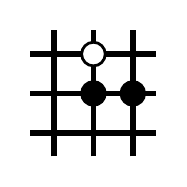
\begin{tikzpicture}
\drawGrid
\drawB{0}{0}
\drawB{1}{0}
\drawW{0}{1}
\end{tikzpicture}
}
edge from parent [gray!50] node[left] {$Q+U$}
}
child {node (select-01) {
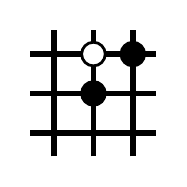
\begin{tikzpicture}
\drawGrid
\drawB{0}{0}
\drawB{1}{1}
\drawW{0}{1}
\end{tikzpicture}
}
child {node (select-010) {
\begin{tikzpicture}[white]
\drawGrid
\end{tikzpicture}
}
edge from parent node[left] {$\max$}
}
child {node (select-011) {
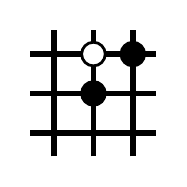
\begin{tikzpicture}
\drawGrid
\drawB{0}{0}
\drawB{1}{1}
\drawW{0}{1}
\end{tikzpicture}
}
edge from parent [gray!50] node[right] {$Q+U$}
}
edge from parent node[right] {$Q+U$}
node[left] {$\max$}
};
\end{tikzpicture}
};
\end{scope}

\begin{scope}
\node[font=\LARGE] (expand-eval-label) at (9,0) {扩展与评估};
\node[below=0.5 of expand-eval-label,xshift=0.7cm] (expand-eval) {
\begin{tikzpicture}
\node (expand-eval-0) {
\begin{tikzpicture}
\drawGrid
\drawB{0}{0}
\drawW{0}{1}
\end{tikzpicture}
}
child {node (expand-eval-00) {
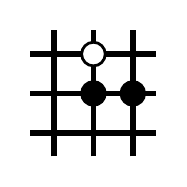
\begin{tikzpicture}
\drawGrid
\drawB{0}{0}
\drawB{1}{0}
\drawW{0}{1}
\end{tikzpicture}
}
edge from parent [gray!50] node[left] {$P$}
}
child {node (expand-eval-01) {
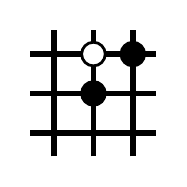
\begin{tikzpicture}
\drawGrid
\drawB{0}{0}
\drawB{1}{1}
\drawW{0}{1}
\end{tikzpicture}
}
child {node (expand-eval-010) {
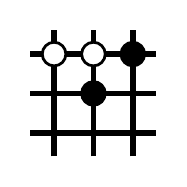
\begin{tikzpicture}
\drawGrid
\drawB{0}{0}
\drawB{1}{1}
\drawW{0}{1}
\drawW{-1}{1}    
\end{tikzpicture}
}
child {node (expand-eval-0100) {
\begin{tikzpicture}[white]
\drawGrid
\end{tikzpicture}
}
edge from parent [black] node[left] {$P$}
}
child {node (expand-eval-0101) {
\begin{tikzpicture}[white]
\drawGrid
\end{tikzpicture}
}
edge from parent [black] node[right] {$P$}
}
edge from parent [gray!50] node[left] {$P$}
}
child {node (expand-eval-011) {
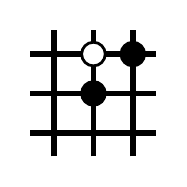
\begin{tikzpicture}
\drawGrid
\drawB{0}{0}
\drawB{1}{1}
\drawW{0}{1}
\end{tikzpicture}
}
edge from parent [gray!50] node[right] {$P$}
}
edge from parent [gray!50] node[right] {$P$}
};
\end{tikzpicture}
};
\node at (6,-8.5) {$(p,v)=f_\theta$};
\node (p) at (5.18,-8.55) {\phantom{$p$}};
\node (P-label) at (7.82,-9.64) {\phantom{$P$}};
\draw[->,-{Latex[length=3mm, width=4mm]},line width=4,rounded corners=0.2cm] (p) |- (P-label);
\end{scope}

\begin{scope}[edge from parent/.style={draw, {Latex[length=3mm, width=4mm]}-, line width=4},]
\node[font=\LARGE] (update-label) at (18,0) {更新};
\node[below=0.5 of update-label,xshift=0.55cm] (update) {
\begin{tikzpicture}
\node (update-0) {
\begin{tikzpicture}
\drawGrid
\drawB{0}{0}
\drawW{0}{1}
\end{tikzpicture}
}
child {node[label={[xshift=0.2cm]left:\textcolor{gray!50}{$v$}}]  (update-00) {
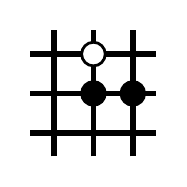
\begin{tikzpicture}
\drawGrid
\drawB{0}{0}
\drawB{1}{0}
\drawW{0}{1}
\end{tikzpicture}
}
edge from parent [gray!50] node[left] {$Q$}
}
child {node[label={[xshift=0.2cm]left:\textcolor{Orchid}{$v$}}]  (update-01) {
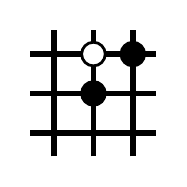
\begin{tikzpicture}
\drawGrid
\drawB{0}{0}
\drawB{1}{1}
\drawW{0}{1}
\end{tikzpicture}
}
child {node[label={[xshift=0.2cm]left:\textcolor{TealBlue}{$v$}}]  (update-010) {
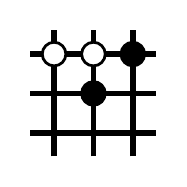
\begin{tikzpicture}
\drawGrid
\drawB{0}{0}
\drawB{1}{1}
\drawW{0}{1}
\drawW{-1}{1}    
\end{tikzpicture}
}
edge from parent [TealBlue] node[left] {$Q$}
}
child {node[label={[xshift=0.2cm]left:\textcolor{gray!50}{$v$}}] (update-011) {
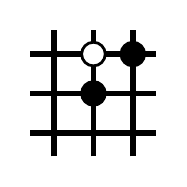
\begin{tikzpicture}
\drawGrid
\drawB{0}{0}
\drawB{1}{1}
\drawW{0}{1}
\end{tikzpicture}
}
edge from parent [gray!50] node[right] {$Q$}
}
edge from parent [Orchid] node[right] {$Q$}
};
\end{tikzpicture}
};
\end{scope}

\begin{scope}
\node[font=\LARGE] (cal-pi-label) at (27,0) {计算$\pi$};
\node[below=0.5 of cal-pi-label] (cal-pi) {
\begin{tikzpicture}
\node (cal-pi-0) {
\begin{tikzpicture}
\drawGrid
\drawB{0}{0}
\drawW{0}{1}
\end{tikzpicture}
};
\end{tikzpicture}
};
\node[below=0.1 of cal-pi,label={[yshift=-1cm]\textcolor{gray}{$\alpha_\theta$}}] (tree) {
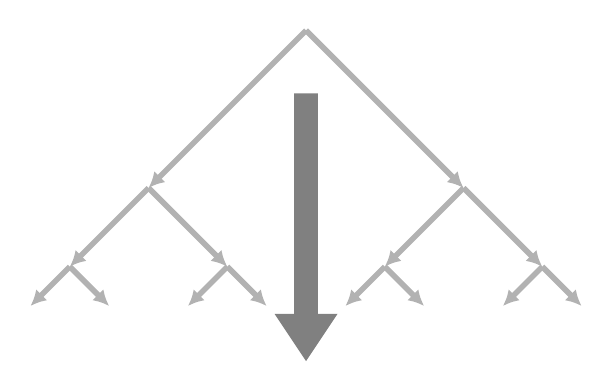
\begin{tikzpicture}
\drawTree
\end{tikzpicture}
};
\node[below=0.1 of tree,label=below:$\pi$] (pi) {

\begin{tikzpicture}[scale=0.2]
    \randDistThree;
\end{tikzpicture}
};
\end{scope}

\draw[->,-{Latex[length=4mm, width=6mm]},line width=6,shorten <= 0.35cm, shorten >=0.35cm] (select-label) -- (expand-eval-label);
\draw[->,-{Latex[length=4mm, width=6mm]},line width=6,shorten <= 0.35cm, shorten >=0.35cm] (expand-eval-label) -- (update-label);
\draw[->,-{Latex[length=4mm, width=6mm]},rounded corners=0.2cm,line width=6,shorten <= 0.35cm, shorten >=0.35cm] (update-label) -- ++(0,2) -- ++(-18,0) -- (select-label);
\draw[rounded corners=0.2cm,line width=4,dash pattern=on 0pt off 2\pgflinewidth,line cap=round,gray!60] (-3,3) rectangle (22.5,-11);
\draw[->,-{Latex[length=4mm, width=6mm]},line width=6,shorten <= 4.35cm, shorten >=0.35cm] (update-label) -- (cal-pi-label);
\end{tikzpicture}
\end{document}
